\documentclass[uplatex,dvipdfmx]{jsarticle}
\usepackage{amssymb}
\usepackage{amsmath}
\usepackage{amsthm}
\usepackage{framed}
\usepackage{braket}
\usepackage{bm}
\usepackage{mathrsfs}
\usepackage{accents}
\usepackage{tocloft}
\usepackage[dvipdfmx]{graphicx}
\usepackage{tikz}
\usepackage{url}
\usepackage{color}
\usepackage{xifthen}
\usepackage{xcolor}
\usepackage{framed}
\usepackage{mathtools}
\usepackage[explicit]{titlesec}
\usepackage{geometry}
\geometry{left=35mm,right=35mm,top=35mm,bottom=35mm}

\usetikzlibrary{positioning}
\usetikzlibrary{calc}
\usetikzlibrary{decorations.pathreplacing}
\usetikzlibrary{cd}

\newcommand{\scrN}{\mathcal{N}}
\newcommand{\scrC}{\mathcal{C}}
\newcommand{\scrI}{\mathcal{I}}
\newcommand{\scrJ}{\mathcal{J}}
\newcommand{\N}{\mathbb{N}}
\newcommand{\Z}{\mathbb{Z}}
\renewcommand{\P}{\mathbb{P}}
\newcommand{\B}{\mathbb{B}}
\newcommand{\Q}{\mathbb{Q}}
\newcommand{\R}{\mathbb{R}}
\newcommand{\C}{\mathbb{C}}
\newcommand{\range}{\operatorname{ran}}
\newcommand{\dom}{\operatorname{dom}}
\newcommand{\append}{{}^\frown}
\newcommand{\boldsig}{\boldsymbol{\Sigma}}
\newcommand{\boldpi}{\boldsymbol{\Pi}}
\newcommand{\bolddelta}{\boldsymbol{\Delta}}
\newcommand{\Ordinals}{\mathrm{On}}
\newcommand\forces{\Vdash}
\newcommand\notforces{\nVdash}
\newcommand{\cl}{\operatorname{cl}}
\newcommand{\intr}{\operatorname{int}}
\newcommand{\rank}{\operatorname{rank}}
\newcommand{\Pow}{\mathcal{P}}
\newcommand{\OR}{\mathbin{\text{または}}}
\newcommand{\AND}{\mathbin{\text{かつ}}}
\newcommand{\GP}{\operatorname{GP}}
\newcommand{\non}{\operatorname{non}}
\newcommand{\cov}{\operatorname{cov}}
\newcommand{\add}{\operatorname{add}}
\newcommand{\cof}{\operatorname{cof}}
\newcommand{\nul}{\mathcal{N}}
\newcommand{\meager}{\mathcal{M}}
\newcommand{\frakt}{\mathfrak{t}}
\newcommand{\frakc}{\mathfrak{c}}
\newcommand{\frakb}{\mathfrak{b}}
\newcommand{\frakd}{\mathfrak{d}}
\newcommand{\all}{\mathrm{all}}
\newcommand{\ZFC}{\mathrm{ZFC}}
\newcommand{\ZF}{\mathrm{ZF}}
\newcommand{\AD}{\mathrm{AD}}
\newcommand{\DC}{\mathrm{DC}}
\newcommand{\proj}{\operatorname{proj}}
\newcommand{\cf}{\operatorname{cf}}
\newcommand{\LCU}{\mathsf{LCU}}
\newcommand{\COB}{\mathsf{COB}}
\newcommand{\relR}{\mathbf{R}}

\DeclarePairedDelimiter\abs{\lvert}{\rvert}
\newcommand{\seq}[1]{{\langle#1\rangle}}
\DeclarePairedDelimiterX{\norm}[1]{\lVert}{\rVert}{#1}

\renewcommand\emptyset{\varnothing}
\renewcommand\subset{\subseteq}
\renewcommand{\setminus}{\smallsetminus}


\theoremstyle{definition}
\newtheorem{thm}{定理}
\newtheorem*{thm*}{定理}
\newtheorem{defi}[thm]{定義}
\newtheorem*{defi*}{定義}
\newtheorem{lem}[thm]{補題}
\newtheorem*{lem*}{補題}
\newtheorem{fact}[thm]{事実}
\newtheorem*{fact*}{事実}
\newtheorem{prop}[thm]{命題}
\newtheorem*{prop*}{命題}
\newtheorem{exm}[thm]{例}
\newtheorem*{exm*}{例}
\newtheorem{rmk}[thm]{注意}
\newtheorem*{rmk*}{注意}
\newtheorem{cor}[thm]{系}
\newtheorem*{cor*}{系}
\newtheorem*{notation*}{記法}
\newtheorem{prob}[thm]{問題}
\newtheorem{conj}[thm]{予想}
\renewcommand{\proofname}{証明}


\usepackage[backend=biber,style=alphabetic,sorting=nty,doi=false,isbn=false,url=false,eprint=true]{biblatex}
\addbibresource{cichonsmaximum.bib}
\renewbibmacro{in:}{}

\title{Cichoń's maximumの証明}
\author{後藤 達哉}

\begin{document}
	\maketitle
	
	
	\tableofcontents
	
	\section{イントロダクション}
	
	実数全体の集合$\R$をLebesgue測度0集合たちで覆うには,それらが最低何個必要かという問いを考える.Lebesgue測度0集合の可算和はLebesgue測度0だから可算個では足りない.一方,$\bigcup_{r \in \R} \{r\} = \R$だから連続体濃度個あれば十分である.
	これで非可算かつ連続体濃度以下とわかるわけだが,ここで問いを終えてしまうのはもったいない.連続体濃度の下に非可算基数が存在することもありえると分かっているからだ.
	そこで問の答えを
	\[
	\cov(\nul) = \min \{ \abs{\mathcal{A}}  : \mathcal{A}\text{はルベーグ測度}0\text{集合の族で}\bigcup \mathcal{A} = \R \}
	\]
	とおいて,これがいろんな集合論のモデルでどうなっているのか調べよう.
	また,他の似たような問いの答えを文字でおいてそれらの間の関係を調べよう:ZFCの範囲内で大小関係がつくのか,等しいのか,ZFCで等しいことを証明できないなら実際にどんなモデルで破れているのか.これが\textbf{基数不変量}の研究である.
	
	基数不変量という言葉に厳密な定義はないが,「実数の構造によって定義される基数」のことである.
	
	いくつかの基数不変量を定義しよう.
	
	$2^\omega$上のイデアル$\mathcal{I}$に対して
	\begin{itemize}
		\item $\add(\mathcal{I}) = \min \{ \abs{\mathcal{J}} : \mathcal{J} \subset \mathcal{I}, \bigcup \mathcal{J} \not \in \mathcal{I}  \}$
		\item $\cov(\mathcal{I}) = \min \{ \abs{\mathcal{J}} : \mathcal{J} \subset \mathcal{I}, \bigcup \mathcal{J} = 2^\omega  \}$
		\item $\non(\mathcal{I}) = \min \{ \abs{A} :  A\subset 2^\omega, A \not \in \mathcal{I} \}$
		\item $\cof(\mathcal{I}) = \min \{ \abs{\mathcal{J}} :  \mathcal{J} \subset \mathcal{I}, (\forall A \in \mathcal{I})(\exists B \in \mathcal{J})(A \subset B) \}$
	\end{itemize}
	とおく.
	これらにルベーグ測度$0$集合のイデアル$\nul$,痩せ集合のイデアル$\meager$を代入したものが考察の対象である.
	
	また,
	\begin{itemize}
		\item $\frakd = \min \{\abs{F} : F \subset \omega^\omega, (\forall f \in \omega^\omega)(\exists g \in F) (f \le^* g) \}$.
		\item $\frakb = \min \{\abs{F} : F \subset \omega^\omega, \neg (\exists f \in \omega^\omega)(\forall g \in F) (g \le^* f) \}$.
	\end{itemize}
	という基数不変量も考えられる.$\frakd$はdominating number,$\frakb$はbounding numberと呼ばれる.
	
	以上の10個の基数不変量のZFCで示せる大小関係については以下の図式が知られていて,Cichońの図式と呼ばれる.
	
	\[
	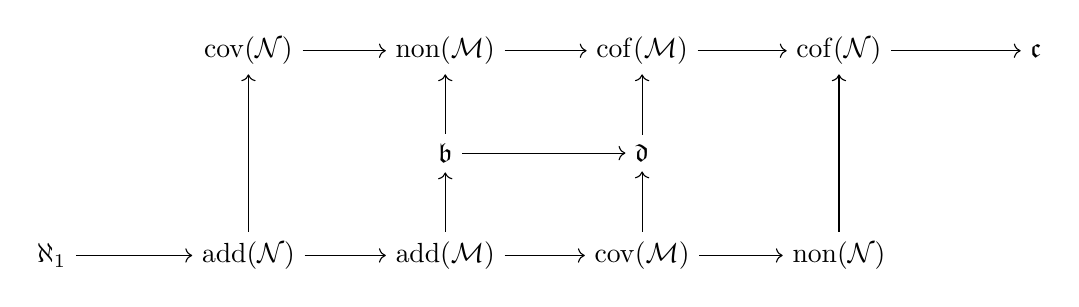
\begin{tikzpicture}
		\newcommand{\w}{2.5}
		\newcommand{\h}{1.3}
		
		\node (aleph1) at (-\w, 0) {$\aleph_1$};
		
		\node (addN) at (0, 0) {$\add(\nul)$};
		\node (covN) at (0, \h*2) {$\cov(\nul)$};
		
		\node (addM) at (\w, 0) {$\add(\meager)$};
		\node (b) at (\w, \h) {$\mathfrak{b}$};
		\node (nonM) at (\w, \h*2) {$\non(\meager)$};
		
		\node (covM) at (\w*2, 0) {$\cov(\meager)$};
		\node (d) at (\w*2, \h) {$\mathfrak{d}$};
		\node (cofM) at (\w*2, \h*2) {$\cof(\meager)$};
		
		\node (nonN) at (\w*3, 0) {$\non(\nul)$};
		\node (cofN) at (\w*3, \h*2) {$\cof(\nul)$};
		
		\node (c) at (\w*4, \h*2) {$\frakc$};
		
		\draw[->] (aleph1) to (addN);
		\draw[->] (addN) to (covN);
		\draw[->] (addN) to (addM);
		\draw[->] (covN) to (nonM);	
		\draw[->] (addM) to (b);
		\draw[->] (b) to (nonM);
		\draw[->] (addM) to (covM);
		\draw[->] (nonM) to (cofM);
		\draw[->] (covM) to (d);
		\draw[->] (d) to (cofM);
		\draw[->] (b) to (d);
		\draw[->] (covM) to (nonN);
		\draw[->] (cofM) to (cofN);
		\draw[->] (nonN) to (cofN);
		\draw[->] (cofN) to (c);
	\end{tikzpicture}
	\]
	ここで矢印$A \to B$は$A \le B$をZFCで証明できることを意味する.
	また$\add(\meager) = \min \{ \cov(\meager), \frakb \}$かつ$\cof(\meager) = \max \{ \non(\meager), \frakd \}$がZFCで証明できる.
	
	Cichońの図式に表示されている基数不変量以外にもBlassの図式と呼ばれる図式の基数不変量:$\mathfrak{m}, \mathfrak{p}, \mathfrak{h}, \mathfrak{g}, \mathfrak{s}, \mathfrak{e}, \mathfrak{r}, \mathfrak{a}, \mathfrak{u}, \mathfrak{i}$などもある.しかし,本稿ではこれらには焦点を当てない.
	
	\begin{table}[p]\label{table:history}
		\caption{Cichońの図式の歴史}
			\begin{tabular}{@{} l|l|p{8cm}}
			年     & 人物                                & 出来事                                                                                                                                                       \\ \hline
			1875年 & du Bois-Reymond & $\aleph_0 < \frakb$の証明 \\ \hline
			1891年 & Cantor & $\aleph_0 < \frakc$の証明 \\ \hline
			1938年 & Rothberger                        & $\cov(\meager) \le \non(\nul)$と$\cov(\nul)\le\non(\meager)$の証明                                                                                            \\ \hline
			1963年 & Cohen                             & 連続体仮説の独立性                                                                                                                                                 \\ \hline
			1970年 & Martin--Solovay                   & Martinの公理およびその帰結の$\add(\nul)=\frakc>\aleph_1$の証明                                                                                                           \\ \hline
			1977年 & Truss                             & $\min\{\cov(\meager), \frakb\} \le \add(\meager)$の証明                                                                                                       \\ \hline
			1981年 & Miller                            & $\add(\meager) \le \min\{\cov(\meager), \frakb\}$の証明およびこの時点で知られていたモデルでのCichonの図式の中の基数不変量の値の決定,Kunen-Millerの表 (5x5マス) \\ \hline
			1984年 & Miller                            & $\add(\nul) \le \frakb$の証明; Kunen-Millerの表 (6x6マス)                                                                                                        \\ \hline
			1984年 & Bartoszyński                      & $\add(\nul) \le \add(\meager)$の証明                                                                                                                         \\ \hline
			1984年 & Fremlin                      & $\cof(\meager) = \max\{\non(\meager), \frakd\}$の証明; Cichoń's diagram登場                                                                                                                     \\ \hline
			1985年 & Raisonnier--Stern                 & $\cof(\meager) \le \cof(\nul)$の証明                                                                                                                         \\ \hline
			1989年 & Bartoszyński--Judah--Shelah       & $\mathrm{PT}_{f,g}$強制法の開発および連続体濃度が$\aleph_2$のときのCichońの図式の分離すべて完成                                                 \\ \hline
			2019年 & Goldstern--Kellner--Shelah         & 巨大基数を仮定したCichoń's maximumの証明                                                                                                                              \\ \hline
			2021年 & Goldstern--Kellner--Mejía--Shelah & 巨大基数を仮定しないCichoń's maximumの証明                                                                                                                             
		\end{tabular}
	\end{table}

	表\ref{table:history}にCichońの図式の歴史をまとめた.
	
	連続体仮説の否定の無矛盾性以前にRothbergerの結果があるのがすごいが,この結果は「Luzin集合とSierpinski集合の両方が存在するならば連続体仮説が成り立つ」という定理の補題として証明された.
	Cantorの$\aleph_0 < \frakc$以前にdu Bois-Reymondが$\aleph_0 < \frakb$を示していたことも驚くべきところであろう.
	
	Kunen-Millerの表というのは図\ref{fig:kunen-miller}のようなものである.\cite{Miller1981SomePO}から抜粋した.Cichońの図式ができる前はどの組合せが可能かこのような表で表していた.
	
	\begin{figure}[p]\label{fig:kunen-miller}
		\begin{center}
		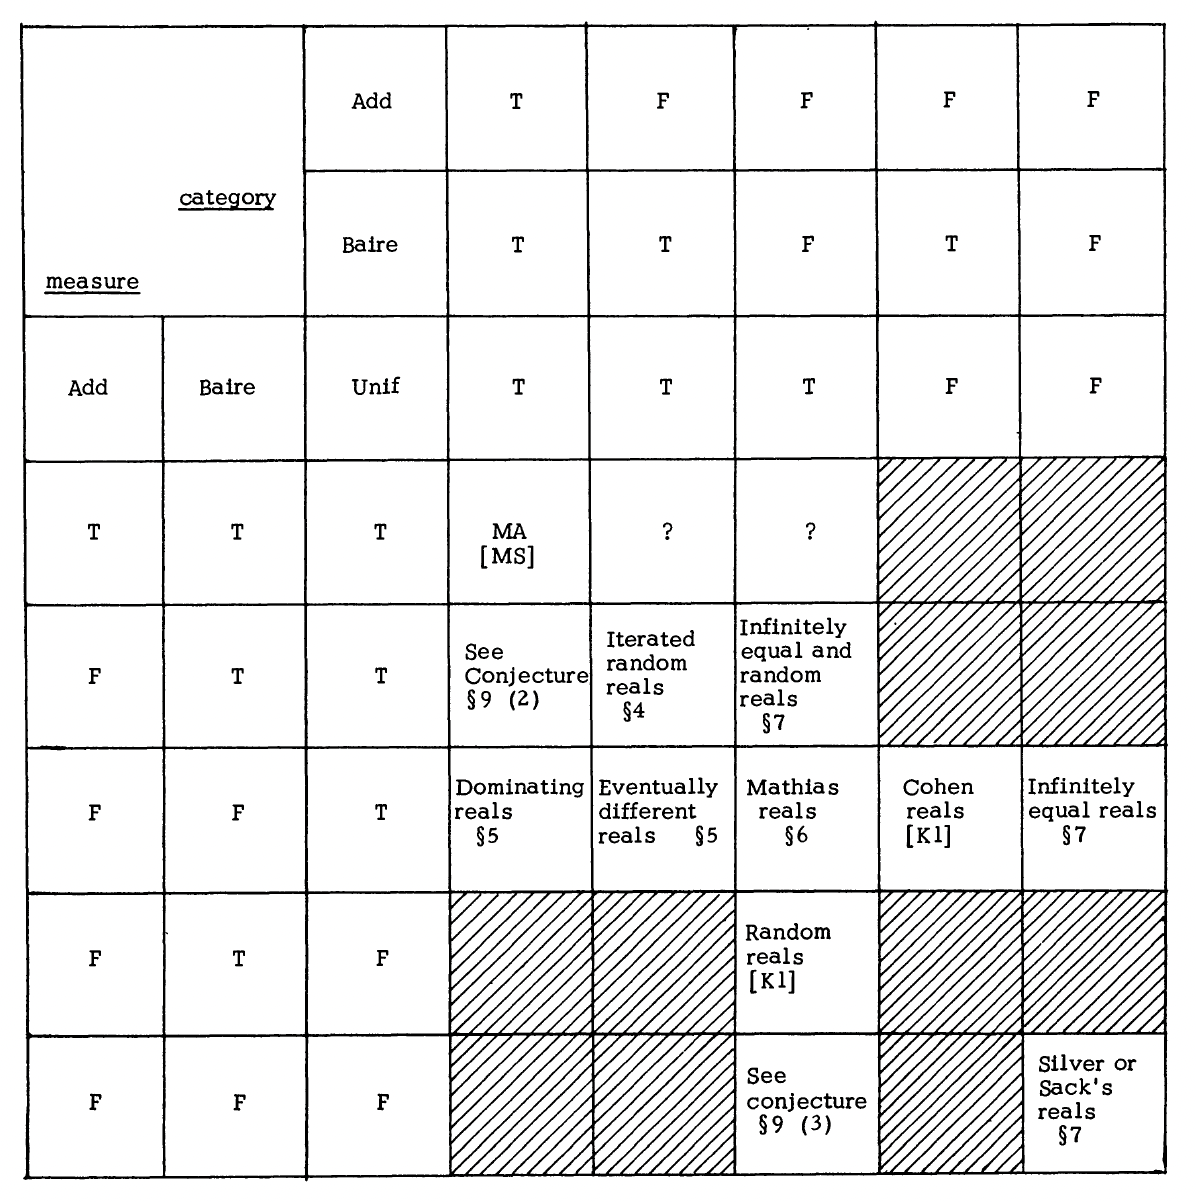
\includegraphics[width=7cm]{kunen-miller.png}
		\caption{Kunen-Millerの表}
		\end{center}
	\end{figure}
	
	表題にもなっているCichoń's maximumであるが,これはCichońの図式において (他の基数不変量の値に束縛されている$\add(\meager), \cof(\meager)$を除いて)すべての基数不変量の値を同時に別々の値にするモデルである.
	そのようなモデルの構成法を本稿では見ていく.
	
	\subsection{relational systems}
	
	\begin{defi}
		\begin{enumerate}
			\item $\mathcal{C} = \{ (q_n)_{n \in \omega}	 : \text{各}q_n\text{は正の有理数かつ} \sum_n q_n \le 1 \}$とおく.
			\item $\Omega_n = \{ a \in [2^{<\omega}]^{<\aleph_0} : \mu(\bigcup_{s \in a} [s]) \le 2^{-n} \}$とおき,$\Omega = \prod_{n \in \omega} \Omega_n$とおく.各$x \in \Omega$について$N_x = \bigcap_{n \in \omega} \bigcup_{s \in x(n)} [s]$とおく.
		\end{enumerate}
	\end{defi}
	
	\begin{defi}
		\begin{enumerate}
			\item $\relR_1 = (\mathcal{C}, \mathcal{C}, \{(x,y) : (\forall^\infty n) (x(n) \le y(n))\})$
			\item $\relR_2 = (\Omega, 2^\omega, \{ (x, y) : y \not \in N_x \})$
			\item $\relR_3 = (\omega^\omega, \omega^\omega, \{ (x,y) : (\forall^\infty n)(x(n) \le y(n))\})$
			\item $\relR_4 = (\omega^\omega, \omega^\omega, \{ (x,y) : (\forall^\infty n) x(n) \ne y(n) \})$
		\end{enumerate}
	\end{defi}

	\begin{lem}
		\begin{enumerate}
			\item $\frakd_{\relR_1} = \cof(\nul), \frakb_{\relR_1} = \add(\nul)$,
			\item $\frakd_{\relR_2} = \non(\nul), \frakb_{\relR_2} = \cov(\nul)$,
			\item $\frakd_{\relR_3} = \frakd, \frakb_{\relR_3} = \frakb$,
			\item $\frakd_{\relR_4} = \cov(\meager), \frakb_{\relR_4} = \non(\meager)$.
		\end{enumerate}
	\end{lem}
	
	\subsection{Cohen,ランダム,Hechler,アメーバ,eventually different強制法}
	
		\subsubsection{Cohen強制法}
		
		$\C = 2^{<\omega}$で順序を延長関係で入れたもの$q \le p \iff p \subset q$はCohen強制法と呼ばれる.
		$\C$ジェネリックフィルター$G$から作られる実数$c = \bigcup G$をCohen実数という.
		Cohen実数から$G$を復元できる:$G = \{ c \upharpoonright n : n \in \omega \}$.
		Cohen強制法は可算なので,明らかに$\sigma$-centeredを満たす.特にcccを満たす.
		
		\subsubsection{ランダム強制法}
		
		$\B = \{ T : T\text{は}2^{<\omega}\text{の部分木で}\mu([T]) > 0 \}$で順序を包含関係で入れたもの$T' \le T \iff T' \subset T$をランダム強制法という.
		$\B$ジェネリックフィルター$G$から作られる実数$r = \bigcap \{[T] : T \in G \}$をランダム実数という.
		ランダム実数から$G$を復元できる:$G = \{ T \in \B : r \in [T] \}$.
		ランダム強制法はcccを満たす.		
		
		\subsubsection{Hechler強制法}
		
		$\mathbb{D} = \{ (n, f) : n \in \omega, f \in \omega^\omega \}$で順序を
		\[(m, g) \le (n, f) \iff n \le m \land f \upharpoonright n = g \upharpoonright n \land (\forall k \in \omega)(f(k) \le g(k))\]
		で入れたものをHechler強制法という.
		$\mathbb{D}$ジェネリックフィルター$G$から作られる実数$d = \bigcup \{ f \upharpoonright n : (n, f) \in G \}$をHechler実数という.
		Hechler実数から$G$を復元できる:$G = \{ (n, f) : f \upharpoonright n = d \upharpoonright n \}$.
		Hechler強制法は$\sigma$-centeredである.
		
		\subsubsection{アメーバ強制法}
		
		$\mathbb{A} = \{ T : T\text{は}2^{<\omega}\text{のsubtreeで}\mu([T])\ge 1/2 \}$で順序を$T' \le T \iff T' \subset T$で入れたものをアメーバ強制法という.
		アメーバ強制法はcccである.
		
		
	\subsection{goodness}
	\subsection{$\LCU$と$\COB$}
	
	\section{Cichońの図式の左半分}
	
	\section{ブール超冪}
	
	\nocite{*}
	\printbibliography[title={参考文献}]
\end{document}